%!TEX root = ./template-skripsi.tex
%-------------------------------------------------------------------------------
%                            BAB III
%               		PEMBAHASAN
%-------------------------------------------------------------------------------

\chapter{HASIL DAN PEMBAHASAN}

Dalam penelitian ini tahapan yang akan dilakukan adalah seperti gambar di bawah ini

\begin{figure}[H]
	\centering
	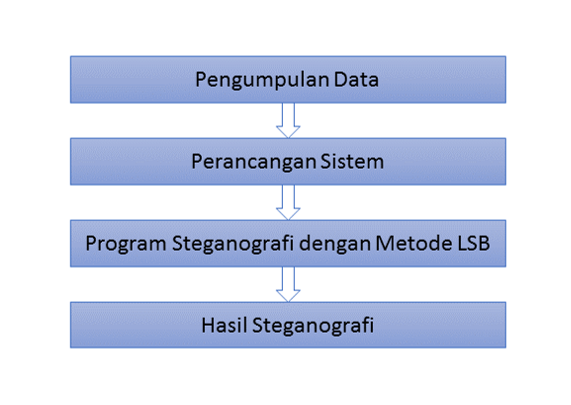
\includegraphics[width=0.8\textwidth]{gambar/alur_penelitian}
	\caption{Alur Penelitian}
	\label{alur_penelitian}
\end{figure}

\section{Pengumpulan Data}
\begin{enumerate}
	\item Studi Pustaka\\
	Penulis mendapatkan informasi yang berkaitan dengan steganografi melalui buku referensi dan juga dalam bentuk \emph{e-book}. Penulis juga mencari informasi melalui berbagai situs di internet yang sesuai dengan topik.	
	\item Studi Literatur\\
	Penulis mencoba mencari perbandingan dengan studi sejenis dari beberapa karya ilmiah lokal maupun internasional, seperti jurnal dan skripsi.	 
\end{enumerate}

\section{Perancangan Sistem}

	\subsection{Proses Penyisipan (\emph{Encoding}) pesan ke Citra \emph{Digital}}
	
	\begin{figure}[H]
		\centering
		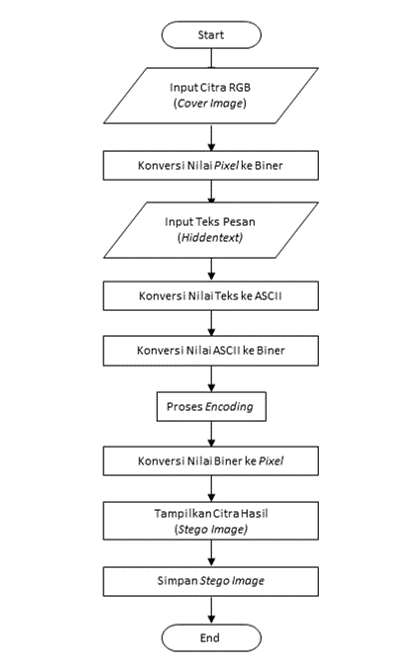
\includegraphics[height=0.8\textheight]{gambar/penyisipan3}
		\caption{\emph{Flowchart} Penyisipan Pesan Rahasia}
		\label{flowchart_penyisipan}
	\end{figure}

	Pada gambar di atas adalah \emph{flowchart} proses penyisipan pesan ke dalam \emph{file}
	citra (\emph{Cover Image}). Dimulai dengan membaca \emph{file} citra RGB. Untuk \emph{file} bitmap 24 bit maka setiap \emph{pixel} (titik) pada gambar tersebut terdiri dari susunan
	tiga warna Merah, Hijau dan Biru (RGB) yang masing-masing disusun oleh bilangan 8 bit
	(1 \emph{byte}) dari 0 sampai 255 atau dengan format biner 00000000 sampai 11111111. Setelah
	membaca \emph{pixel} dari \emph{file} citra langkah selanjutnya menentukan bit terkecil (LSB) pada \emph{Cover Image}.
	
	Selanjutnya adalah menyisipkan pesan (\emph{Hiddentext}) yang akan disembunyikan ke dalam \emph{Cover Image}. Pesan tersebut dikonversi terlebih dahulu menjadi nilai ASCII dan kemudian dikonversi kembali menjadi nilai Biner. Setelah itu terjadilah proses penyisipan (\emph{Encoding}). Selanjutnya biner yang telah disisipkan akan dikonversikan kembali ke dalam \emph{pixel}. Dan menyimpan citra yang telah disisipkan pesan ke dalam \emph{Cover Image} sehingga diperoleh atau	dapat ditampilkan sebuah gambar baru (\emph{Stego Image}).
	
	\subsection{Proses Ekstraksi (\emph{Decoding}) pesan dari Citra \emph{Digital}}
	
	\begin{figure}[H]
		\centering
		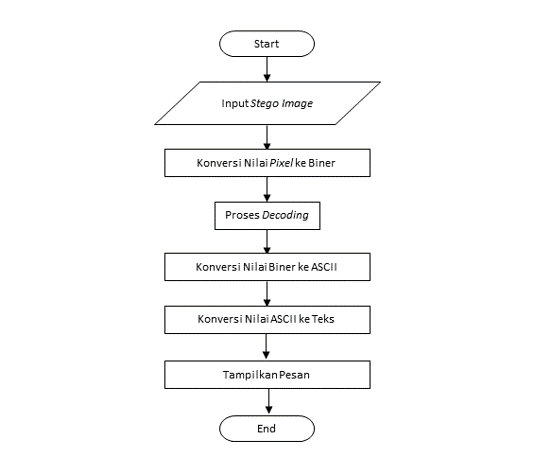
\includegraphics[height=0.6\textheight]{gambar/ekstraksi3}
		\caption{\emph{Flowchart} Ekstraksi Pesan Rahasia}
		\label{flowchart_ekstraksi}
	\end{figure}

	Pada gambar di atas adalah \emph{flowchart} proses ekstraksi pesan dari \emph{Stego Image} yang menghasilkan \emph{Hiddentext} yang terdapat di dalamnya. Prosesnya dimulai dengan
	membaca \emph{file} citra, dan mengubah \emph{pixel} ke dalam nilai biner.
	Kemudian proses ekstraksi (\emph{Decoding}). Setelah diperoleh bit-bit yang tersembunyi pada \emph{Cover Image} maka proses
	berikutnya adalah mengkonversi kembali pesan yang tersembunyi (\emph{Hiddentext}), sehingga pesan dapat ditampilkan kembali.

	\subsection{Desain Antar Muka Program}
	
	Berikut adalah desain antar muka dari program steganografi yang dibangun dengan menggunakan Matlab.
	
	\begin{figure}[H]
		\centering
		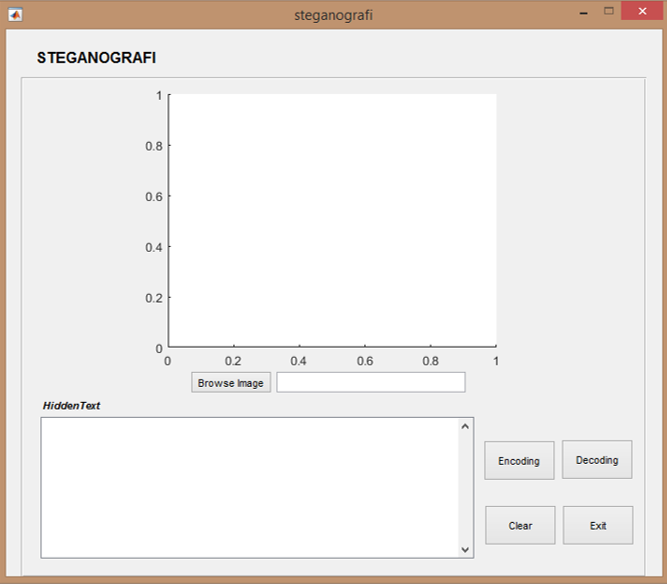
\includegraphics[width=1\textwidth]{gambar/mockup/1}
		\caption{Desain \emph{Form} Steganografi}
		\label{desain_form}
	\end{figure}

	Dari tampilan tersebut, pengambilan gambar yang akan dijadikan sebagai \emph{Cover Image} dilakukan dengan menekan tombol "\emph{Browse Image}" dan gambar akan tampil. 
	
	\begin{figure}[H]
		\centering
		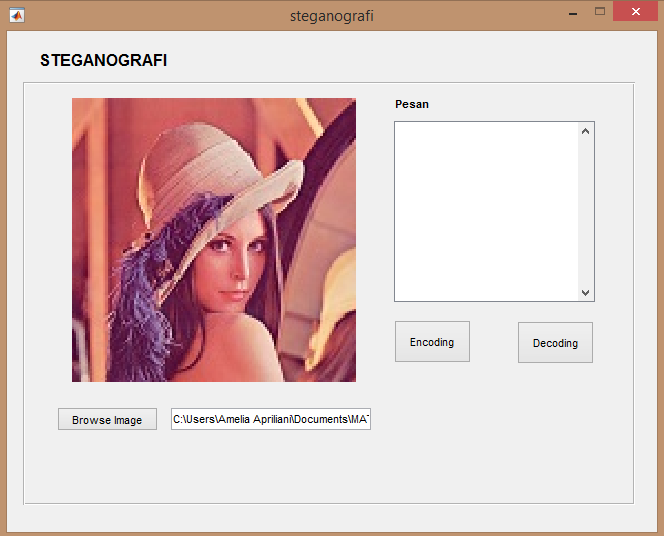
\includegraphics[width=1\textwidth]{gambar/mockup/2}
		\caption{Desain \emph{Form} - \emph{Cover Image}}
		\label{desain_image}
	\end{figure}

	Setelah \emph{Cover Image} tampil maka pesan yang akan disisipkan atau \emph{Hiddentext} dapat dituliskan pada kolom pesan. Dan kemudian klik tombol \emph{Encoding} untuk melakukan proses \emph{Encoding}. Setelah proses \emph{Encoding}, maka akan didapatkan \emph{Stego Image} dan disimpan di folder yang sama.
	
	\begin{figure}[H]
		\centering
		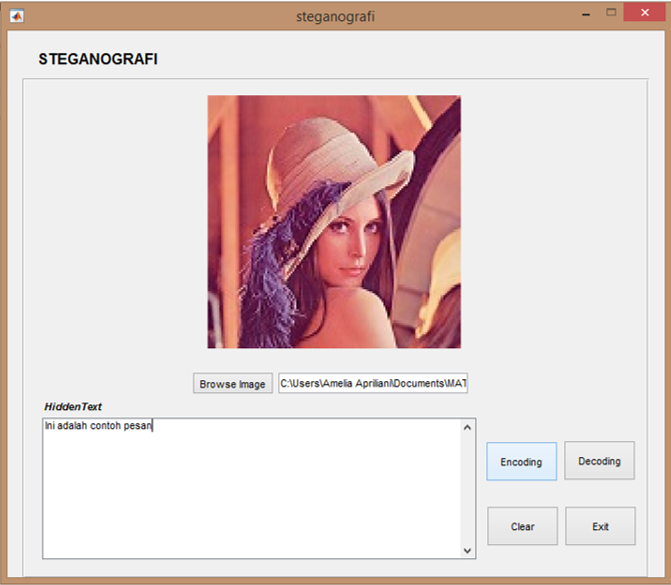
\includegraphics[width=1\textwidth]{gambar/mockup/3}
		\caption{Desain \emph{Form} - Proses \emph{Encoding}}
		\label{desain_encoding}
	\end{figure}

	Jika ingin melakukan proses \emph{Decoding}, maka buka \emph{Stego Image} yang telah disimpan. Kemudian klik tombol \emph{Decoding} dan pesan akan didapatkan.
	
	\begin{figure}[H]
		\centering
		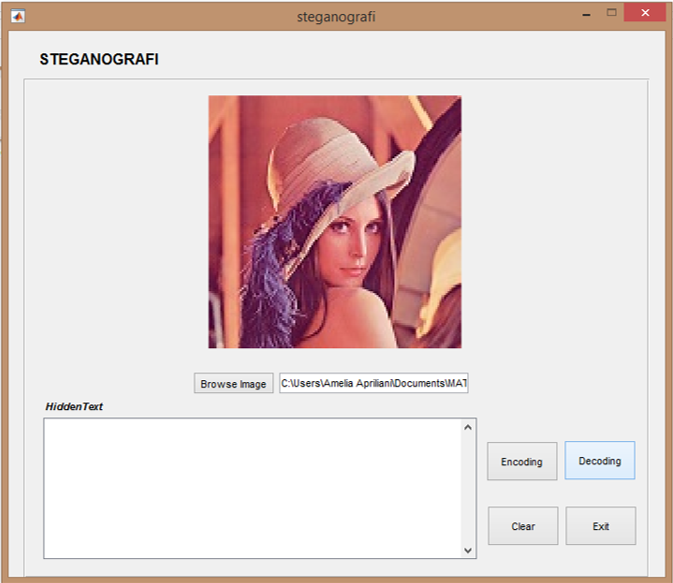
\includegraphics[width=1\textwidth]{gambar/mockup/4}
		\caption{Desain \emph{Form} - Proses \emph{Decoding}}
		\label{desain_decoding}
	\end{figure}

	\begin{figure}[H]
		\centering
		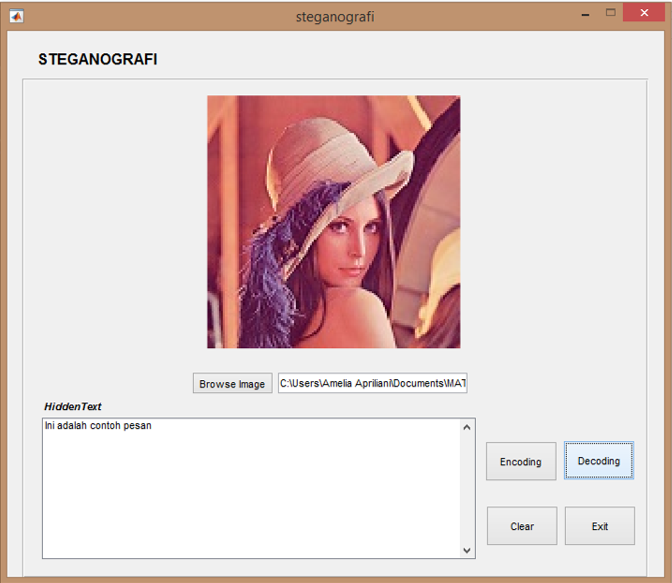
\includegraphics[width=1\textwidth]{gambar/mockup/5}
		\caption{Desain \emph{Form} - Pesan Hasil \emph{Decoding}}
		\label{desain_pesan}
	\end{figure}

\section{Program Steganografi dengan Metode LSB}
Program diawali dengan pengambilan \emph{file} citra \emph{digital} yang akan digunakan, berikut adalah \emph{source code}-nya:
	\begin{figure}[H]
		\centering
		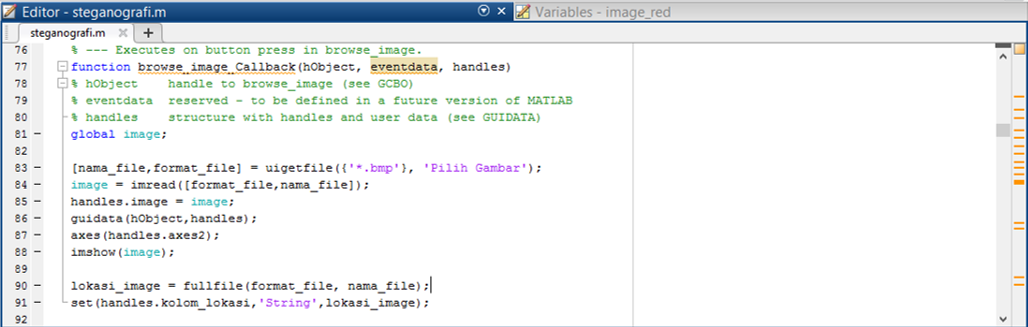
\includegraphics[width=1\textwidth]{gambar/source_code/browse_image}
		\caption{\emph{Source Code} - \emph{Browse Image}}
		\label{browse_image}
	\end{figure}

Selanjutnya adalah memasukkan pesan atau \emph{Hiddentext}. \emph{Hiddentext} yang akan dimasukkan tidak boleh melebihi batas maksimal karakter. Panjang karakter maksimal disesuaikan dengan besar \emph{pixel} pada \emph{file} citra. Panjang karakter maksimal dapat dihitung, berikut adalah \emph{source code}-nya:
	\begin{figure}[H]
		\centering
		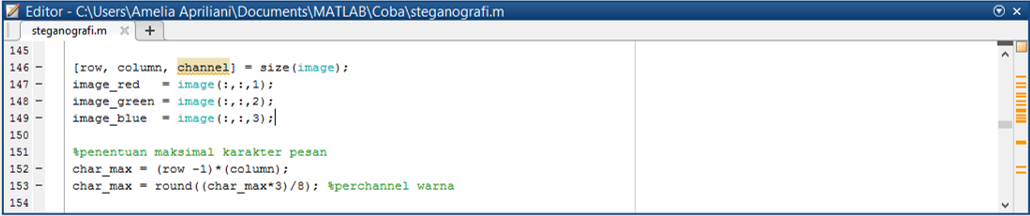
\includegraphics[width=1\textwidth]{gambar/source_code/karakter_maksimal}
		\caption{\emph{Source Code} - Menghitung Karakter Maksimal}
		\label{karakter_max}
	\end{figure}

Sedangkan untuk menghitung panjang \emph{hiddentext} yang telah dimasukkan adalah sebagai berikut:
	\begin{figure}[H]
		\centering
		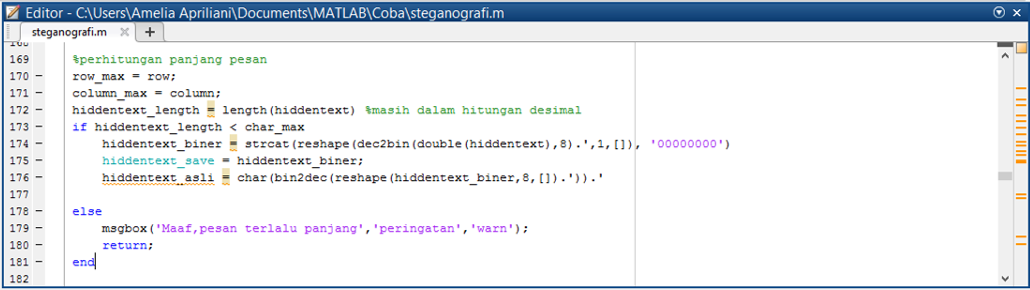
\includegraphics[width=1\textwidth]{gambar/source_code/panjang_pesan}
		\caption{\emph{Source Code} - Menghitung Panjang \emph{Hiddentext} yang Dimasukkan}
		\label{panjang_pesan}
	\end{figure}

\subsection{\emph{Encoding}}
Pada tugas akhir ini metode yang digunakan dalam steganografi adalah metode LSB. Proses \emph{Encoding} merupakan proses penyisipan pesan atau \emph{Hiddentext} ke dalam \emph{file} citra. Berikut adalah cuplikan \emph{source code} proses \emph{Encoding} dengan menggunakan metode LSB:
	\begin{figure}[H]
		\centering
		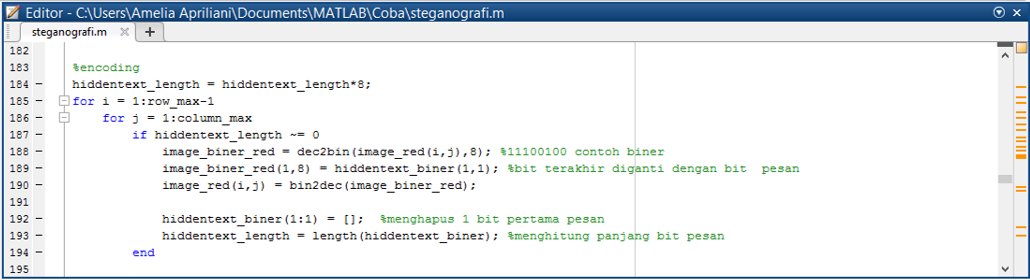
\includegraphics[width=1\textwidth]{gambar/source_code/cuplikan_encoding}
		\caption{\emph{Source Code} - Cuplikan \emph{Encoding}}
		\label{cuplikan_encoding}
	\end{figure}

\subsection{\emph{Decoding}}
Proses \emph{Decoding} merupakan proses pengambilan kembali pesan atau \emph{Hiddentext} yang telah disisipkan ke dalam \emph{file} citra. Berikut merupakan cuplikan dari \emph{source code} proses \emph{Decoding}:
	\begin{figure}[H]
		\centering
		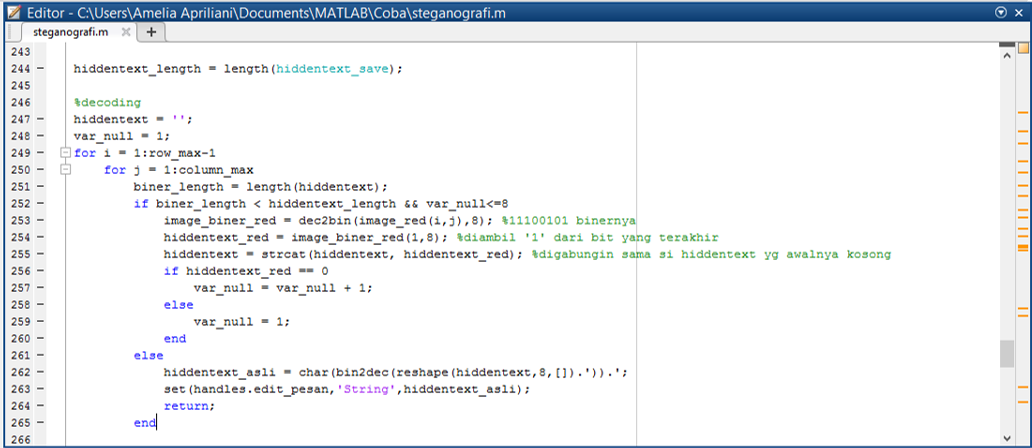
\includegraphics[width=1\textwidth]{gambar/source_code/cuplikan_decoding}
		\caption{\emph{Source Code} - Cuplikan \emph{Decoding}}
		\label{cuplikan_decoding}
	\end{figure}
	
\section{Hasil Steganografi}
Setelah dilakukan pengujian terhadap program Steganografi, maka didapatkan hasil sebagai berikut:
	\subsection{Pengujian Berdasarkan \emph{Imperceptible}}
	Pengujian ini menguji kualitas citra \emph{digital}, apakah citra \emph{digital} akan mengalami perubahan yang mencurigakan atau tidak secara visual. Pengujian ini dikatakan berhasil apabila kualitas dari \emph{Stego Image} yang dihasilkan tidak berbeda jika dibandingkan dengan berkas aslinya atau \emph{Cover Image}.

	%gambar cover
	\begin{figure}[H]
		\centering
		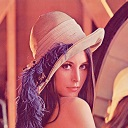
\includegraphics[width=0.75\textwidth]{gambar/matlab/lena}
		\caption{\emph{Cover Image}}
		\label{lena_asli}
	\end{figure}

	%gambar stego
	\begin{figure}[H]
		\centering
		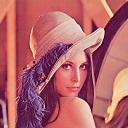
\includegraphics[width=0.75\textwidth]{gambar/matlab/lena_kalimat}
		\caption{\emph{Stego Image}}
		\label{lena_pesan}
	\end{figure}

	\subsection{Pengujian Berdasarkan \emph{Fidelity}}
	Pengujian ini berdasarkan proses penyembunyiaan pesan atau \emph{Encoding}. Pada proses penyembunyian pesan dapat berhasil apabila ukuran pesan yang akan disembunyikan sesuai dengan kapasitas \emph{file} citra. Apabila ukuran pesan melebihi kapasitas maksimal dari \emph{file} citra, maka program tidak akan melanjutkan proses \emph{Encoding}. Kapasitas pesan dipengaruhi oleh ukuran \emph{pixel} dari citra \emph{digital}. Semakin besar ukuran \emph{pixel} dari citra \emph{digital}, maka semakin besar pula kapasitas pesan yang bisa disembunyikan.
	
	%masukkin tabel
	\begin{table}[H]
		\centering
		\caption{Hasil Proses \emph{Encoding}}
		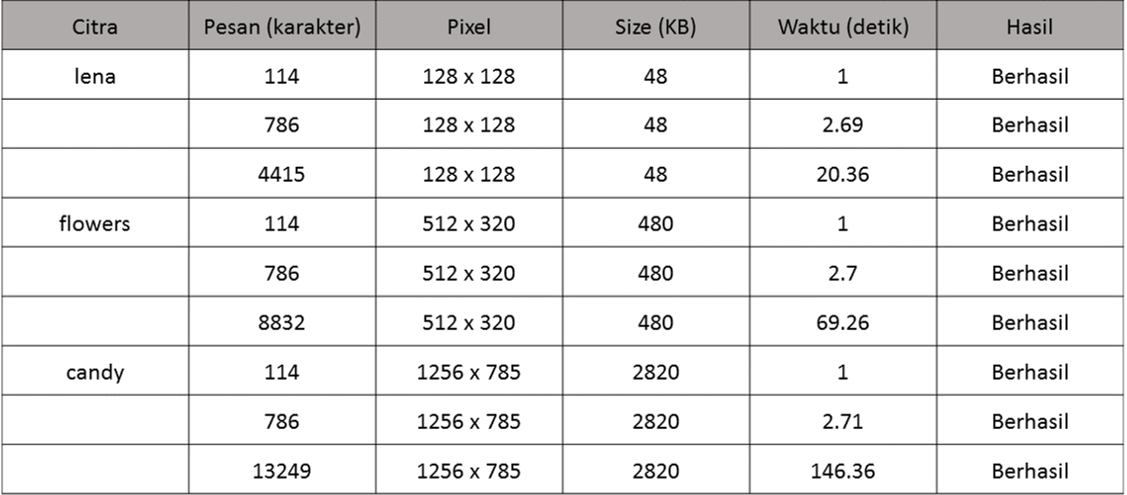
\includegraphics[width=1.0\textwidth]{gambar/table_hasilencode}
		\label{tabel_hasilencode2}
	\end{table}
	
	\subsection{Pengujian Berdasarkan \emph{Recovery}}
	Pengujian ini berdasarkan proses ektraksi pesan atau \emph{Decoding}. Untuk membuktikan apakah program steganografi ini berhasil, maka harus dapat dibuktikan bahwa pesan di dalam \emph{Stego Image} dapat diambil kembali. Jika pengujian dilakukan dengan benar, maka \emph{Hiddentext} dapat ditampilkan sesuai dengan yang dimasukkan. 
	
	Pada penelitian ini, pesan yang dihasilkan dari proses \emph{Decoding} tidak menghasilkan karakter-karakter aneh yang tidak dapat dibaca. Hasil dari pengujian ekstraksi pesan dapat dilihat pada tabel 3.2
	 
	%masukkin tabel
	\begin{table}[H]
		\centering
		\caption{Hasil Proses \emph{Decoding}}
		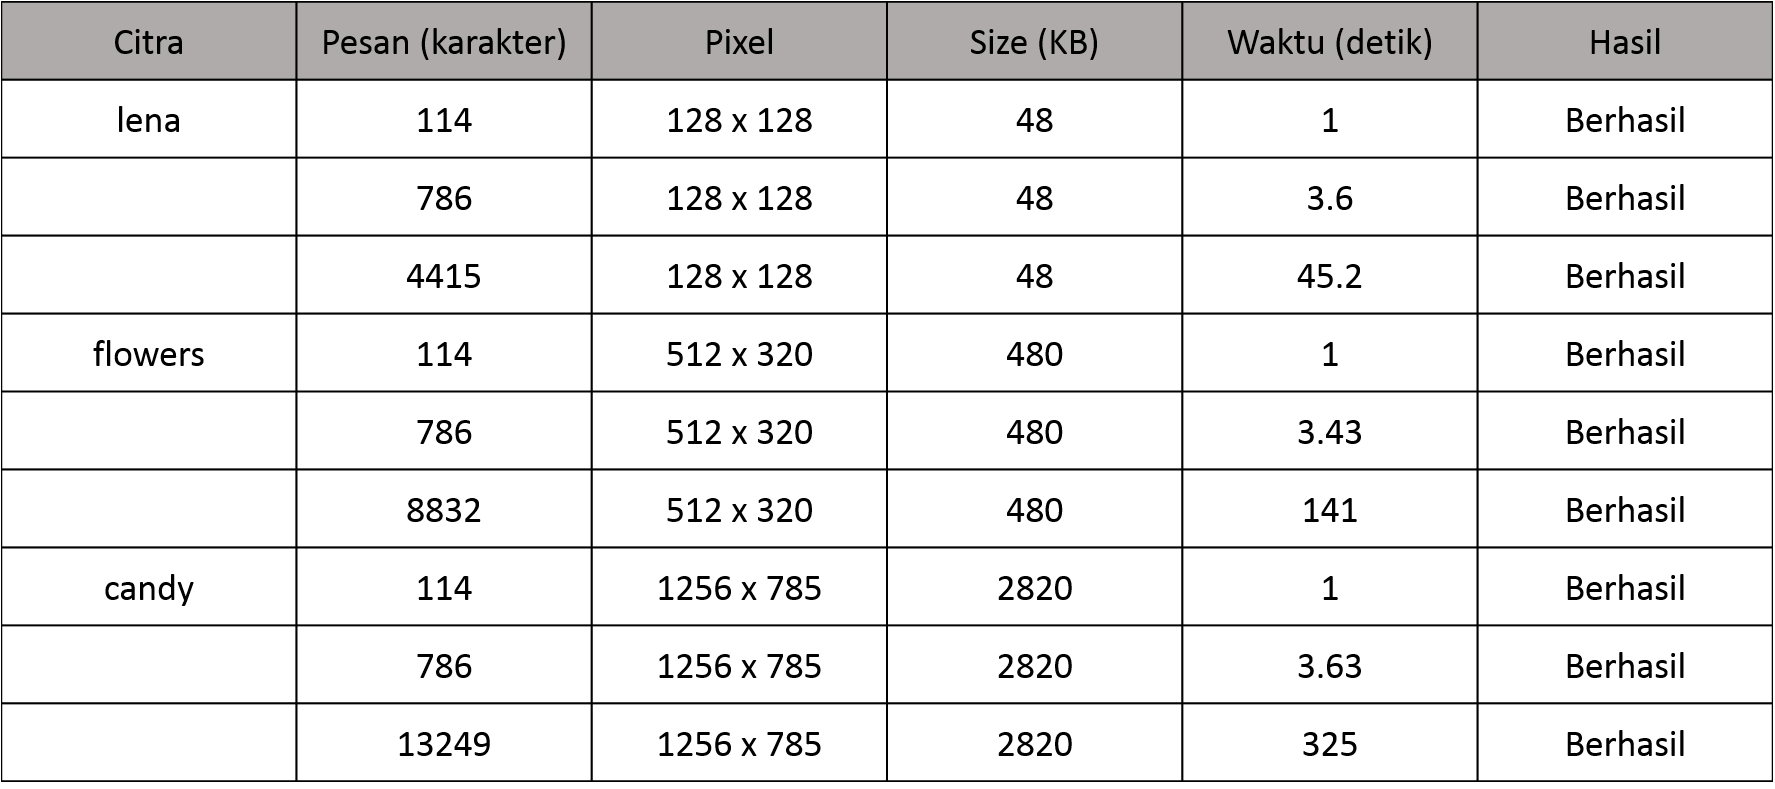
\includegraphics[width=1.0\textwidth]{gambar/table_hasildecode2}
		\label{tabel_hasildecode2}
	\end{table}
	
	\subsection{Kesimpulan Pengujian}
	